\subsection*{Las 7 emociones básicas}
Las emociones evolucionaron para cumplir la función de promover la supervivencia física, pero el desarrollo de la cultura humana también ha impulsado la evolución de las emociones en el sentido de que estas cumplan funciones relativas a metas sociales, tales como llevarse bien con los demás y avanzar en la comunidad. Las emociones básicas tienen funciones sociales además de las de supervivencia \cite{rulicki2012cnv}.

Estas siete emociones básicas son:
\begin{itemize}
\item \textbf{Alegría:} Sensación dichosa de placer y bienestar \cite{rulicki2012cnv}.
\item \textbf{Tristeza:} Sensación opresiva de pérdida o carencia que produce desánimo \cite{rulicki2012cnv}.
\item \textbf{Miedo:} Sensación de agitación causada por una percepción de peligro debida a riesgos físicos, morales, o la presencia de dolor \cite{rulicki2012cnv}.
\item \textbf{Enojo:} Sensación perturbadora que resulta de una ofensa, una torpeza propia o un obstáculo natural. Generalmente incluye el deseo de reaccionar agresivamente \cite{rulicki2012cnv}.
\item \textbf{Asco:} Sensación de repugnancia debida a la percepción de un estímulo desagradable a los sentidos \cite{rulicki2012cnv}.
\item \textbf{Desprecio:} Sensación de rechazo o desestimación hacia otra persona o cosa, por considerarla inferior, indigna o carente de valor \cite{rulicki2012cnv}.
\item \textbf{Sorpresa:} Sensación súbita e inesperada de asombro \cite{rulicki2012cnv}.
\end{itemize}

\subsubsection*{Las señales faciales de las emociones}
Las señales faciales son las configuraciones de los distintos rasgos particulares de cada emoción, que son producidas por movimientos involuntarios en los músculos del rostro. Según Ekman, las expresiones de las emociones nos dan información acerca de lo que está ocurriendo dentro de la persona, lo que posiblemente ocurrió antes de que se desarrollara la emoción y aquello que puede llegar a pasar en consecuencia de la emoción \cite{ekman2017rostro}.

\begin{figure}[t]
    \centering
    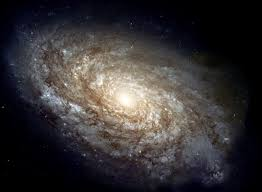
\includegraphics[width=0.5\textwidth]{galaxia.jpg}
    \caption{Una imagen de una galaxia.}
    \label{fig:mesh1}
\end{figure}

\begin{table}[b]
\centering
\begin{tabular}{|c|c|c|c|}
\hline
\textbf{item} & \textbf{característica 1} & \textbf{característica 2} & \textbf{característica 3} \\ \hline
1             & 3234                      & 12323                     & 4343                      \\ \hline
2             & 1332                      & 123123                    & 12                        \\ \hline
3             & 1232                      & 4334                      & 12312                     \\ \hline
\end{tabular}
\caption{Tabla generada automáticamente.}
    \label{cuadro:prueba2}
\end{table}

